\documentclass[]{article}
\usepackage{aale}
\usepackage{graphicx}
\usepackage{booktabs}
\usepackage{url}

\title{Factory Control Unit}
\runningtitle{Factory Control Unit}
\subtitle{Modellgetriebene, vollständig KI-generierte Steuerung für die Lernfabrik Factory-in-a-Box}

\author{1}{Klaus M. Liebler}
\affil{1}{Hochschule Osnabrück, Fakultät für Ingenieurwissenschaften und Informatik, Osnabrück, Deutschland}

\confno{23}
\confdate{17.--19. März\ }
\confyear{2027}
\confplace{Fulda}

\logofile{logo}

\begin{document}
\setcounter{page}{1}
\maketitle

\abstract{Lernfabriken machen Automatisierungstechnik greifbar und werden an berufsbildenden Schulen und Hochschulen für angewandte Wissenschaften in praxisorientierten Lehrformaten eingesetzt. Factory-in-a-Box (FiaB) ist eine kompakte, mobile und kostengünstige Open-Source-Lernfabrik. Der Beitrag skizziert die aktuelle Ausbaustufe von FiaB und stellt anschließend die Factory Control Unit (FCU) vor, die eingebettete Zentralsteuerung der Anlage. Im Mittelpunkt steht ihre Software. Sie wurde vollständig von einem KI-Codierassistenten geschrieben, gesteuert von einem einzelnen erfahrenen Entwickler. Beschrieben werden das Vorgehen (Best-in-Class-Analyse bestehender Open-Source-Komponenten, konsequente Nutzung von C++26, dreistufige Testkette aus Host-, QEMU- und Renode-Tests), das so entstandene Echtzeitbetriebssystem rtoos mit eigenen, gehärteten Kommunikationsstacks für OPC UA, Modbus, EtherCAT und HTTPS/WebSocket sowie eine IEC-61131-3-Programmierumgebung mit Visualisierung, die vollständig im Browser läuft. Abschließend werden die Folgen dieser Art der Softwareentwicklung für Lehre und Forschung diskutiert.}

\keywords{Factory-in-a-Box, Lernfabrik, Eingebettete Systeme, KI-gestützte Softwareentwicklung, IEC 61131-3, OPC UA}


\section{Einleitung und Stand der Technik}\label{sec:intro}

Für die berufliche Bildung und die Hochschullehre existiert eine Reihe kommerzieller Lehraufbauten. Die fischertechnik Training Factory~\cite{fischertechnik} bildet Abläufe eines Industrieunternehmens mit Baukastenkomponenten nach, nutzt industrietypische Technik jedoch kaum. Festo Didactic und, stärker auf einzelne Regelkreise ausgerichtet, GUNT bieten modulare, industrienahe Systeme an, deren Anschaffungskosten von typischerweise 20.000\,€ bis über 100.000\,€ eine Mehrfachbeschaffung für Kleingruppen kaum zulassen. Deutlich günstiger (ca.~6.000\,€) ist das an den Berufsbildenden Schulen Osnabrück entwickelte Smart Factory Model~\cite{strating2023}, bei dem eine reale SPS einen kompakten Portalroboter steuert. Factory-in-a-Box (FiaB)~\cite{liebler2025} ist eine kompakte, mobile und kostengünstige Open-Source-Modellfabrik, die auf der Experimentierplattform Lab@Home~\cite{liebler2023} aufbaut. Sie ist Teil des Vorhabens X-in-a-boX~\cite{xinabox2025}, das Lehraufbauten für Kleinladungsträger mit einem Zielbudget von unter 1.000\,€ entwickelt, die autark betrieben und bei Bedarf sicher in ein Hochschulnetz eingebunden werden können.

Naheliegend ist die Frage, warum FiaB nicht direkt von einer handelsüblichen SPS gesteuert wird. Die Factory Control Unit (FCU) ersetzt die SPS nicht. Sie übernimmt die Rolle, die in einer realen Anlage dezentrale Peripherie und intelligente Feldgeräte spielen: Sie bindet Sensoren und Aktoren an und stellt sie über industrieübliche Schnittstellen bereit, nämlich OPC UA~\cite{iec62541}, Modbus TCP und RTU~\cite{modbus} sowie EtherCAT~\cite{ethercat}. Die Steuerungslogik kann damit auf jeder SPS oder Soft-SPS laufen, etwa CODESYS oder TwinCAT; Studierende lernen herstellerunabhängig das Prinzip und nicht ein einzelnes Werkzeug. Schrittmotoren mit sensorlosem Referenzieren, Wägezelle, Farb- und Abstandssensoren, adressierbare RGB-LEDs, Bus-Servos des Roboters und USB Power Delivery ließen sich an einer Kompakt-SPS nur mit zahlreichen Zusatzmodulen anbinden, und der Kostenrahmen wäre nicht zu halten. Zusätzlich bringt die FCU eine eigene IEC-61131-3-Laufzeit mit (Kapitel~\ref{sec:plc}), sodass FiaB auch ohne externe Steuerung betrieben werden kann.

Gegenüber der Kurzfassung hat sich der Schwerpunkt verschoben. Die Firmware basiert nicht mehr auf Eclipse ThreadX~\cite{threadx}, sondern auf dem neu entstandenen Echtzeitbetriebssystem rtoos; hinzugekommen ist die IEC-61131-3-Programmierumgebung. Einer Anregung der Gutachter folgend konzentriert sich der Beitrag auf die Software und auf die Frage, wie sie mit KI-Unterstützung entstanden ist. Kapitel~\ref{sec:fiab} und~\ref{sec:hw} fassen Anlage und Hardware knapp zusammen, Kapitel~\ref{sec:sw} beschreibt Vorgehen und Architektur von rtoos, Kapitel~\ref{sec:plc} die Programmierumgebung. Kapitel~\ref{sec:ki} ordnet die Ergebnisse ein, Kapitel~\ref{sec:lehre} skizziert den Einsatz in der Lehre.

\section{Factory-in-a-Box in der aktuellen Version}\label{sec:fiab}

In FiaB werden in einem Kreislaufprozess aus farbigen Holzklötzen kundenindividuelle Türme gefertigt. Ein 6-DOF-Roboter (RoArm-M3) entnimmt die Klötze einem Durchlaufregal und setzt sie auf einer Montageplattform zu Türmen zusammen; Förderband, Sortier- und Hubachse mit Schrittmotoren, Wägezelle sowie Farb- und Abstandssensoren schließen den Kreislauf. Der mechanische Aufbau folgt weitgehend~\cite{liebler2025}. Neu ist ein Pneumatiksystem, das die Klötze auf das Förderband legt und den bisherigen Servoantrieb ersetzt. Es bildet zugleich eine Druckregelstrecke aus Kompressor, Druckbehälter, einem realen Verbraucher (Doppelkolbenzylinder), drei zuschaltbaren simulierten Verbrauchern (Ventile mit Drossel) und einem Drucksensor. Der Greifer des Roboters wurde durch einen Vakuumsauger ersetzt, was die Prozessrobustheit deutlich erhöht. RGB-LED-Streifen in den senkrechten Stützen dienen als Störmeldeleuchte oder visualisieren Prozessgrößen unmittelbar.

\section{Hardware der Factory Control Unit}\label{sec:hw}

Die wachsende Zahl von Komponenten und der Bedarf an neuen Kommunikationsschnittstellen erforderten es, von Lab@Home~\cite{liebler2023} als zentraler Steuerung abzurücken. Die FCU ist eine vierlagige Platine von etwa 19\,$\times$\,8\,cm, die direkt an den oberen Streben von FiaB verschraubt wird. Die Revisionen 1 und 2 nutzen einen STM32H563 (Cortex-M33, 250\,MHz, 640\,KiB RAM), Revision 3 einen STM32H743 (Cortex-M7, 400\,MHz). Vorhanden sind Ethernet, USB-C als Device-Schnittstelle, ein USB-Power-Delivery-Sink, ein Leistungsmonitor (INA226), FDCAN, ein SD-Karten-Steckplatz und ein EtherCAT-Slave-Controller (LAN9253). Zur Anbindung der Anlage dienen zwei Schrittmotortreiber (TMC2209), ein Wägezellenwandler (HX711), Ausgänge für RGB-LEDs, ein analoger Eingang für den Drucksensor, drei I\textsuperscript{2}C-Busse, MOSFET-PWM-Ausgänge, Eingänge für Lichtschranken sowie serielle TTL-Schnittstellen für den Roboter und einen weiteren Fahrroboter. Die Unterseite trägt alle SMD-Bauteile, die der Leiterplattenfertiger bestückt; die Oberseite enthält die von Hand zu bestückenden Steckverbinder. Die Versorgung erfolgt wahlweise über ein 24-V-Netzteil oder ein USB-PD-Netzteil (20\,V, 100\,W). Alle Unterschiede zwischen den Revisionen sind in der Software in einem Board-Paket gekapselt; der übrige Code ist für alle Revisionen identisch.

\section{Software: KI-gestützte Entwicklung von rtoos}\label{sec:sw}

\subsection{Vorgehen}

Die gesamte Software der FCU, also das Echtzeitbetriebssystem rtoos, die Anwendungsfirmware, die Weboberfläche, die IEC-61131-3-Umgebung, die Emulatormodelle, die Testskripte und die Build-Werkzeuge, wurde von einem KI-Codierassistenten (Claude Code~\cite{claudecode}) geschrieben. Der Autor hat keine Zeile davon selbst verfasst. Seine Aufgaben waren Anforderungen und Architekturentscheidungen, die Formulierung der Aufträge (Prompting), die Bewertung von Zwischenergebnissen und die Inbetriebnahme der Hardware. Die Entwicklung folgte vier Grundsätzen.

Erstens bestand der erste Auftrag nicht darin, Code zu schreiben, sondern etablierte Open-Source-Echtzeitbetriebssysteme und Kommunikationsstacks auf ihre jeweils besten Eigenschaften zu untersuchen. So stammen das Preemption-Threshold-Scheduling und die Block-Pools aus ThreadX~\cite{threadx}, die schlanken Task-Notifications aus FreeRTOS. Die Testsuiten von lwIP, NetX Duo, FreeRTOS-Plus-TCP, TinyUSB, USBX und open62541~\cite{open62541} wurden ausgewertet und ihre Testfälle portiert, allein 309 aus open62541.

Zweitens wurde ohne Rücksicht auf ältere Compiler oder Bibliotheken ausschließlich C++26 (GCC 16) verwendet, und zwar gezielt mit Sprachmitteln, die auf eingebetteten Systemen kompakten Code und möglichst viele Prüfungen zur Übersetzungszeit ermöglichen. Der Hardwarezugriff erfolgt nur über Concepts (statischer Polymorphismus ohne Laufzeitkosten), sodass derselbe Code auf dem Mikrocontroller und auf dem PC läuft. Die Konfiguration jeder Peripherie ist ein Template-Argument; Registerwerte, Teiler und Vorteiler berechnet der Compiler und prüft sie per \texttt{static\_assert} gegen die Grenzen des Referenzhandbuchs. Auch die Pinbelegung wird zur Übersetzungszeit gegen die Pin-Datenbank des Herstellers geprüft, und die sigmoidförmigen Beschleunigungsrampen der Schrittmotoren berechnet der Compiler. Vorbedingungen sind C++26-Contracts~\cite{p2900}, die auf dem PC mit voller Prüfung und auf dem Ziel als schlanke Trap ausgewertet werden. \texttt{std::inplace\_vector} ersetzt dynamische Container, und \texttt{\#embed} bindet Zertifikate und die komprimierte Weboberfläche direkt ins Binärabbild ein. Heap, Exceptions und RTTI werden nicht verwendet. Die vollständige Netzwerk-Firmware mit HTTPS, Modbus und OPC UA belegt rund 217\,KiB RAM plus 52\,KiB DMA-Speicher von 640\,KiB.

Drittens wurden die Errata-Sheets aller unterstützten Prozessorfamilien (STM32H5, H7, G4, F1) von Beginn an in die Entwicklung einbezogen und systematisch gegen jeden Treiber abgeglichen. 18 Errata werden im Code umgangen, jeweils dokumentiert mit Fundstelle und, wo möglich, einem Host-Test; die übrigen sind als nicht zutreffend oder begründet akzeptiert vermerkt. Viertens wurde jede Funktion in einer dreistufigen Testkette abgesichert, die im nächsten Abschnitt beschrieben ist.

\subsection{Dreistufige Testkette}

Auf der ersten Stufe laufen Host-Tests mit GoogleTest auf dem PC: Der Kernel arbeitet auf einem simulierten CPU-Port, der IP-Stack über simulierte Leitungen und der USB-Stack gegen einen simulierten Host. 886 Testfälle in 140 Testgruppen prüfen die gesamte Logik in wenigen Sekunden; nach jedem Netzwerktest wird zusätzlich geprüft, dass alle Paketpuffer an den Pool zurückgegeben wurden. Die zweite Stufe führt den Kernel in einer eigens erstellten QEMU-Maschine~\cite{qemu} auf dem emulierten Cortex-M aus und prüft Kontextwechsel, verzögertes Sichern der FPU-Register, Interrupt-Prioritäten und die Stack-Limit-Überwachung. Die dritte Stufe sind Systemtests in Renode~\cite{renode}: Die unveränderte Firmware läuft dort mit Modellen der Peripherie und ist über einen virtuellen Netzwerkadapter mit dem PC verbunden. Wo die mitgelieferten Renode-Modelle zu ungenau waren, etwa bei SPI und I\textsuperscript{2}C ohne Busdauer, bei Timern ohne Vergleichsausgänge oder bei SDMMC ohne internes DMA, entstanden eigene Modelle, ebenso für INA226 und HX711. Ein Ende-zu-Ende-Test prüft DHCP, DNS, mDNS, SNTP, den TLS-Handshake samt Zertifikatsprüfung, die Weboberfläche, WebSocket, Modbus TCP, OPC UA mit einem unabhängigen Client (asyncua) und das SSH-Terminal mit OpenSSH, auch unter Last. Lücken eines Emulators werden im Modell geschlossen oder ausdrücklich als nicht unterstützt markiert; Tests werden nie abgeschwächt.

Diese Testkette hatte eine bemerkenswerte Folge: Der Autor konnte mit dem vollständigen System bereits über die Weboberfläche im Browser arbeiten und die Wirkungen auf dem Terminal und an den simulierten Ausgängen beobachten, bevor die reale Hardware verfügbar war. Die erstmals auf die Platine geflashte Firmware funktionierte mit nur geringen Einschränkungen.

\begin{figure}[tbp]
\centering
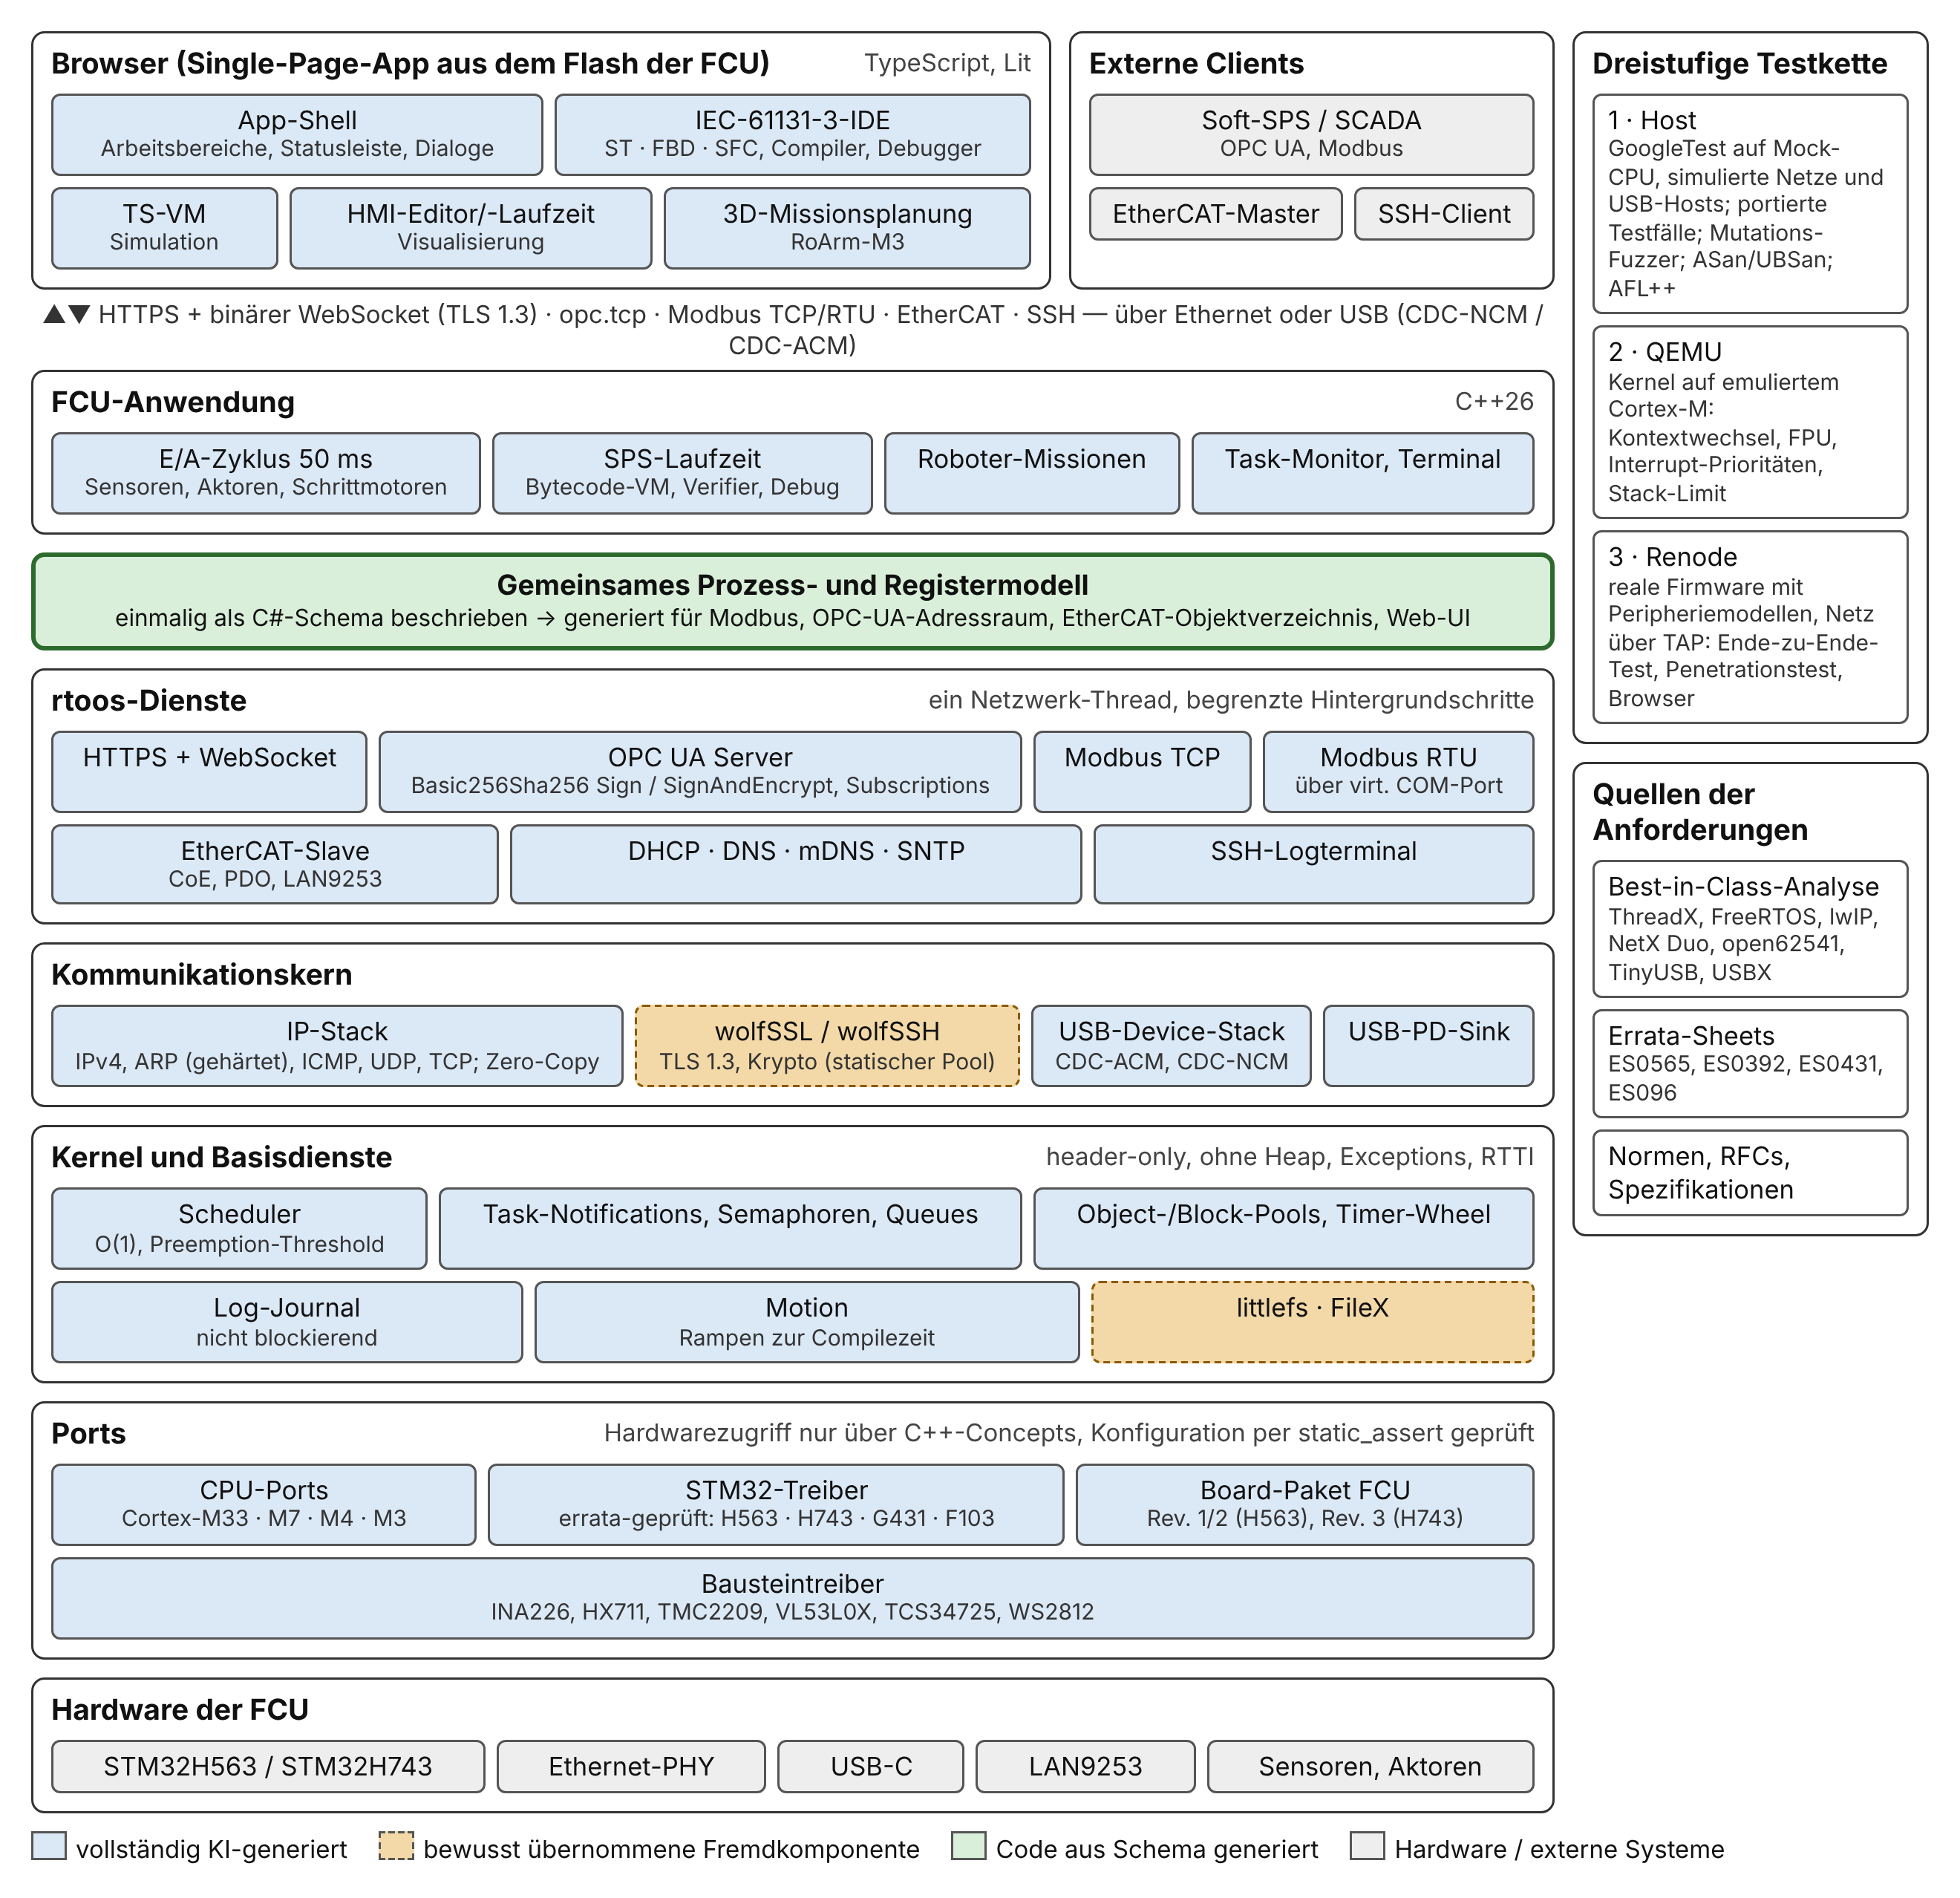
\includegraphics[width=\linewidth]{fig_rtoos_architektur.png}
\caption{Architektur von rtoos und der FCU-Firmware. Blau: vollständig KI-generiert; orange: bewusst übernommene Fremdkomponenten; grün: aus dem Informationsmodell generierter Code.}
\label{fig:arch}
\end{figure}

\subsection{Architektur und Eigenschaften von rtoos}

Bild~\ref{fig:arch} zeigt die Schichten von rtoos und der FCU-Firmware. Die wesentlichen Eigenschaften sind:
\begin{itemize}
\item Kernel: präemptiv mit festen Prioritäten, O(1)-Bereitliste, Preemption-Threshold, Task-Notifications, Semaphoren, Message-Queues, Objekt- und Block-Pools, Timer-Wheel und ein nicht blockierendes Log-Journal. Interrupts oberhalb der Kernel-Maske haben keine zusätzliche Latenz.
\item Ports für Cortex-M33, M7, M4 und M3 sowie für STM32H563, H743, G431 und F103 mit gemeinsamen Treibern für die gleiche Peripherie-IP der Familien.
\item Eigener IP-Stack (IPv4, ARP, ICMP, UDP, TCP, DHCP-Client und -Server, DNS, mDNS, SNTP) mit mehreren Schnittstellen und Paketpuffern ohne Kopieren (Zero-Copy).
\item Eigener USB-Device-Stack mit CDC-ACM (virtueller COM-Port) und CDC-NCM (Ethernet über USB) sowie ein USB-Power-Delivery-Sink.
\item Ein einziger Netzwerk-Thread für alle Dienste: Aufwendige Arbeit wie TLS-Handshakes oder RSA-Operationen läuft in begrenzten Hintergrundschritten, sodass kurze Anfragen nicht warten. Sperren zwischen Servern entfallen; die Fairness wird auf der Leitung getestet.
\item Entscheidungen auf Basis von Messungen: Ein eigener Zero-Copy-TLS-Record-Layer brachte nur 3 bis 6 \% und wurde zugunsten des gepflegten wolfSSL-Codes verworfen; der statische Speicherpool von wolfSSL schrumpfte nach Messung unter Volllast von 208\,KiB auf 72\,KiB.
\end{itemize}

Der Umfang verdeutlicht die Produktivität: rtoos umfasst rund 42.000 Zeilen C++ im Produktivcode, rund 20.000 Zeilen Tests und rund 9.000 Zeilen Emulatormodelle und Testskripte; hinzu kommen etwa 6.500 Zeilen C++ der FCU-Anwendung und 28.000 Zeilen TypeScript für Weboberfläche und Programmierumgebung. Der erste Commit von rtoos ist auf den 25. Oktober 2026 datiert.

\subsection{Kennzahlen}

Tabelle~\ref{tab:kennzahlen} fasst Laufzeit, Speicherbedarf und Testabdeckung zusammen. Die Laufzeiten stammen aus einer eigenen Benchmark-Firmware, die mit dem Zyklenzähler \texttt{DWT\_CYCCNT} je 1000 Durchläufe misst. Sie wurden bisher nur in Renode und QEMU erhoben; beide führen einen Befehl pro Takt bei 250\,MHz aus. Die Werte sind daher Befehlszahlen und keine Taktzyklen; die Umrechnung in Mikrosekunden ist eine Näherung, auf der Hardware kommen Flash-Wartezyklen hinzu. QEMU und Renode stimmen auf wenige Befehle überein. Die Testabdeckung wurde mit gcov über die Host-Tests ermittelt und umfasst nur die 145 Quelldateien, die diese Tests einbinden; Chip-Treiber, die nur auf dem Ziel laufen, prüft der Selbsttest im Emulator, ohne dass ihre Abdeckung gemessen wird.

\begin{table}[htbp]
\centering
\small
\caption{Kennzahlen von rtoos (Laufzeiten: Mittelwerte in Renode, Befehle bei CPI 1 und 250\,MHz).}
\label{tab:kennzahlen}
\begin{tabular}{p{0.50\linewidth}p{0.30\linewidth}p{0.12\linewidth}}
\toprule
\textbf{Kenngröße} & \textbf{Wert} & \textbf{ca.~Zeit} \\
\midrule
Thread durch Task-Notification geweckt & 300 Befehle & 1,2 \textmu s \\[2pt]
Semaphore freigeben, wartender Thread läuft & 339 Befehle & 1,4 \textmu s \\[2pt]
Interrupt bis benachrichtigter Thread läuft & 334 Befehle & 1,3 \textmu s \\[2pt]
Interrupt bis Handler (ohne Kernel-Sperre) & 6 Befehle & 24 ns \\[2pt]
Queue-Rundlauf über zweiten Thread & 729 Befehle & 2,9 \textmu s \\[2pt]
Block-Pool belegen und freigeben & 118 Befehle & 0,5 \textmu s \\[2pt]
Modbus: 10 Holding-Register lesen (PDU) & 403 Befehle & 1,6 \textmu s \\[2pt]
Modbus: 125 Holding-Register lesen (PDU) & 1736 Befehle & 6,9 \textmu s \\[2pt]
Kernel und CPU-Port (Code) & ca.~4,4\,KiB Flash &  \\[2pt]
Kernel-Benchmark, Abbild gesamt & 11,9\,KiB Flash, 12,6\,KiB RAM &  \\[2pt]
Netzwerk-Firmware (HTTPS, Modbus, OPC UA) & 295\,KiB Flash (ohne Testdatei), 269\,KiB RAM &  \\[2pt]
Vollständige FCU-Firmware & ca.~740\,KiB Flash, 475\,KiB RAM &  \\[2pt]
Host-Testfälle & 886 (alle bestanden) &  \\[2pt]
Abdeckung Zeilen / Funktionen / Zweige & 87,1 \% / 92,9 \% / 67,3 \% &  \\[2pt]
\bottomrule
\end{tabular}
\end{table}

\subsection{Gemeinsames Prozessmodell und Kommunikation}

Das Prozessabbild der Anlage ist einmalig als annotierte C\#-Klassen beschrieben. Attribute legen Zugriffsrecht, Einheit, Registeradresse, Wertebereich und Darstellungsart fest. Der Generator UniversalRegisterAccess erzeugt daraus die Registerkonstanten für Modbus, den OPC-UA-Adressraum als constexpr-Tabelle im Flash, das EtherCAT-Objektverzeichnis samt Gerätebeschreibung (ESI) für TwinCAT und die Registerkarte der Weboberfläche. OPC UA (Basic256Sha256 mit Sign oder SignAndEncrypt, Sessions, Browse, Subscriptions), EtherCAT (CoE mit SDO, SDO-Information und PDO-Zuordnung), Modbus TCP und Modbus RTU greifen so auf dasselbe Register- und Prozessmodell zu. Modbus RTU läuft über den virtuellen COM-Port der USB-Schnittstelle, Modbus TCP über das Netzwerk. IP-Verbindungen sind sowohl über Ethernet als auch über den CDC-NCM-Adapter möglich: Ein USB-Kabel genügt, der PC erhält seine Adresse vom DHCP-Server der FCU. Für Praktika zu Hause oder in Räumen ohne Netzinfrastruktur ist das ein wesentlicher Vorteil.

Die Weboberfläche ist eine Single-Page-Anwendung im Applikationslook (Lit, Vite) mit Arbeitsbereichen für Übersicht, Register, Aktoren, Schrittmotoren, Druckregelstrecke, Leistungsmessung, Tasks, System, Terminal und die 3D-Missionsplanung des Roboters, mit Statusleiste, Dialogen, Dunkelmodus und Vollbild. Sie wird Brotli-komprimiert aus dem Flash der FCU ausgeliefert. Danach laufen alle Daten über einen binären WebSocket; Kodierer und Dekodierer für C++ und TypeScript erzeugt ein zweiter Generator aus einem Nachrichtenschema. Statt JSON-Strukturen zyklisch abzufragen, werden nur kompakte Binärnachrichten ausgetauscht.

\subsection{Sicherheit und Härtung}

Alle Kommunikationsstacks sind Bestandteil von rtoos und nutzen Verschlüsselung, soweit das jeweilige Protokoll sie vorsieht: HTTPS und WebSocket ausschließlich mit TLS 1.3, OPC UA mit Basic256Sha256 und das Log-Terminal mit SSH und Public-Key-Anmeldung. Kryptographie und TLS stammen aus wolfSSL~\cite{wolfssl}. Dies ist eine der wenigen Komponenten, die bewusst nicht von der KI nachentwickelt wurden: Sicherheitskritischer Code wird dort von Spezialisten gepflegt und bei Schwachstellen zeitnah korrigiert. Eine projekteigene Zertifizierungsstelle mit Namensbeschränkung auf .local-Namen und private Adressbereiche stellt die Gerätezertifikate aus; OPC-UA-Clients müssen ein Zertifikat dieser Stelle vorweisen, ohne Sicherheit ist nur Lesen erlaubt. Der IP-Stack lernt ARP-Einträge bewusst abweichend von RFC 826 nur aus Antworten auf eigene Anfragen und ist so gegen ARP-Spoofing gehärtet.

Geprüft wird automatisiert auf mehreren Wegen. Die Host-Tests enthalten gezielte Angriffsfälle (fehlerhafte Header, Überlauf von Sequenznummern, SYN-Flut, ARP-Spoofing). Deterministische Mutationsfuzzer für alle Parser laufen in jedem Testlauf mit. Unter Linux laufen alle Host-Tests zusätzlich mit AddressSanitizer und UndefinedBehaviorSanitizer, und AFL++~\cite{aflpp} fuzzt HTTP, WebSocket, DNS, DHCP, Modbus, OPC UA, den EtherCAT-Slave und den Verifier der SPS; eine einstündige Kampagne mit rund 437 Millionen Ausführungen blieb nach den Korrekturen ohne Befund. Schließlich greift ein Black-Box-Penetrationstest die reale Firmware in Renode über das Netz an: Portscan, veraltete TLS-Versionen, Verbindungen, die den Handshake nie abschließen (Slowloris), fehlerhafte HTTP-, WebSocket-, Modbus- und OPC-UA-Nachrichten, mDNS-Kompressionsschleifen und -Verstärkung sowie übergroße ICMP-Pakete. Nach jeder Gruppe wird geprüft, dass das Gerät weiterhin antwortet und nie neu gestartet ist. Tabelle~\ref{tab:befunde} zeigt eine Auswahl der Befunde. Die beiden Fehler in wolfSSL zeigen, dass auch bewusst übernommene Fremdkomponenten von der Testkette profitieren. Die Weboberfläche ist durch eine Anmeldung geschützt: Jede Platine erhält bei der Erstprogrammierung ein eigenes Einmalpasswort, das zusammen mit der Board-ID auf ein Etikett gedruckt wird; das Gerät speichert nur einen PBKDF2-Hash. Sitzungen laufen über ein 256-Bit-Cookie mit Zeitlimit, vier Rollen vom Beobachter bis zum Administrator werden für jede WebSocket-Nachricht geprüft, kritische Aktionen verlangen zusätzlich eine Sitzung über die USB-Schnittstelle als Nachweis physischer Präsenz. Fehlversuche werden pro Adresse und global gedrosselt und protokolliert; der Penetrationstest enthält dafür eine eigene Testgruppe.

\begin{table}[htbp]
\centering
\small
\caption{Gefundene und behobene Schwachstellen (Auswahl) und das Verfahren, das sie aufgedeckt hat.}
\label{tab:befunde}
\begin{tabular}{p{0.22\linewidth}p{0.52\linewidth}p{0.20\linewidth}}
\toprule
\textbf{Komponente} & \textbf{Befund} & \textbf{Aufgedeckt durch} \\
\midrule
WebSocket-Dekodierer & 64-Bit-Länge eines Fortsetzungsrahmens überlief die Größenprüfung; Schreiben hinter den Puffer möglich & AFL++ (30 min) \\[2pt]
HTTPS-Server & Verbindungen ohne abgeschlossenen Handshake sperrten die Weboberfläche aus (Slowloris) & Penetrationstest in Renode \\[2pt]
wolfSSL 5.9.4, RSA-OAEP & Freigabe einer Stack-Adresse in den statischen Pool bei der gewählten Konfiguration & Pool-Zähler im Host-Test \\[2pt]
wolfSSL 5.9.4, RSA-Entschlüsselung & Überlappendes memcpy & AddressSanitizer \\[2pt]
SPS-Lader & Ungeprüftes Befehlsbudget aus dem Abbild blockierte die VM für Minuten & AFL++ \\[2pt]
\bottomrule
\end{tabular}
\end{table}

\section{IEC-61131-3-Programmierumgebung im Browser}\label{sec:plc}

Die FCU lässt sich selbst als SPS programmieren, ohne dass auf dem PC eine Software installiert werden muss. Unterstützt werden Strukturierter Text (ST), Funktionsbausteinsprache (FBS) und Ablaufsprache (AS) als Teilmenge von IEC 61131-3 Ed. 3~\cite{iec61131}; Kontaktplan und Anweisungsliste sowie die objektorientierten Erweiterungen sind bewusst ausgenommen, ein Sicherheitsanspruch (SIL) wird nicht erhoben. Die Entwicklungsumgebung besteht aus einem ST-Editor, grafischen Editoren für FBS und AS, Projektbaum, E/A-Sicht und Beobachtungsliste. Der Compiler (Lexer, Parser, semantische Analyse, Zwischendarstellung, Codeerzeugung) ist in TypeScript geschrieben und läuft im Browser. Das Gerät erhält nur das fertige Abbild aus Bytecode und Debug-Informationen.

Eine zentrale Entscheidung war, Bytecode für eine virtuelle Maschine zu erzeugen statt nativen Maschinencode. Haltepunkte und Einzelschritt werden damit trivial, weil der Zustand der VM in einer Datenstruktur liegt. Jeder Speicherzugriff wird gegen die Segmentgrenzen geprüft, der Rücksprungstapel liegt außerhalb des Datensegments, und ein Befehlsbudget pro Zyklus wirkt als deterministischer Watchdog. Ein fehlerhaftes Programm stoppt so nur die SPS, nicht die Firmware. Derselbe Bytecode läuft auf Cortex-M33 und M7, auf dem PC und im Browser. Der Preis ist eine geringere Geschwindigkeit; abgeschätzt sind mindestens 5 Millionen Bytecode-Befehle pro Sekunde, ein typisches Lehrprogramm benötigt damit weniger als 1\,ms des 50-ms-E/A-Zyklus.

Bild~\ref{fig:sfc} zeigt den AS-Editor mit einer Sortierablaufkette. Der Befehlssatz ist einmal definiert; daraus werden die C++- und die TypeScript-Seite generiert. Die C++-VM ist Teil von rtoos, die TypeScript-VM dient im Browser zur Simulation ohne Hardware. Differenzielle Tests führen einen gemeinsamen Korpus von ST-Programmen auf beiden VMs aus und verlangen byteidentische Verläufe aller Variablen. Der Lader prüft jedes Abbild (Prüfsumme, Bezug zum E/A-Modell, Signaturen der nativen Funktionen) und wurde mit AFL++ gefuzzt. Auf dem Gerät läuft das Programm nach jedem E/A-Zyklus, startet nach dem Einschalten selbstständig und benötigt keinen geöffneten Browser. Ein Umschalter der Steuerquelle legt fest, ob die Ausgänge vom IEC-Programm oder über Modbus, OPC UA und Weboberfläche geschaltet werden, niemals von beiden: Schreibversuche werden dann mit einer Modbus-Exception oder \texttt{Bad\_NotWritable} abgewiesen. Die Online-Fehlersuche bietet Live-Werte, Schreiben und Forcen, Haltepunkte, Einzelschritt sowie aktive AS-Schritte und Signalwerte im FBS live. Neben der Standardbibliothek gibt es eine FCU-Bibliothek und eine Bibliothek nach VDI 3814~\cite{vdi3814}.

Zum Projekt gehört eine Visualisierung. Im Editor werden Seiten gestaltet und ihre Elemente über Variablenpfade an SPS-Variablen gebunden. Die Laufzeit ist eine eigene Seite der Weboberfläche mit Meldeliste und Linienschreibern, die auch im Vollbild auf einem Bedien-PC läuft. Die Seiten werden mit dem Projekt auf der SD-Karte der FCU gespeichert. Damit steht an einer Anlage für unter 1.000\,€ die komplette Kette aus Programmierung, Simulation, Inbetriebnahme, Fehlersuche und Bedienen und Beobachten zur Verfügung.

\begin{figure}[tbp]
\centering
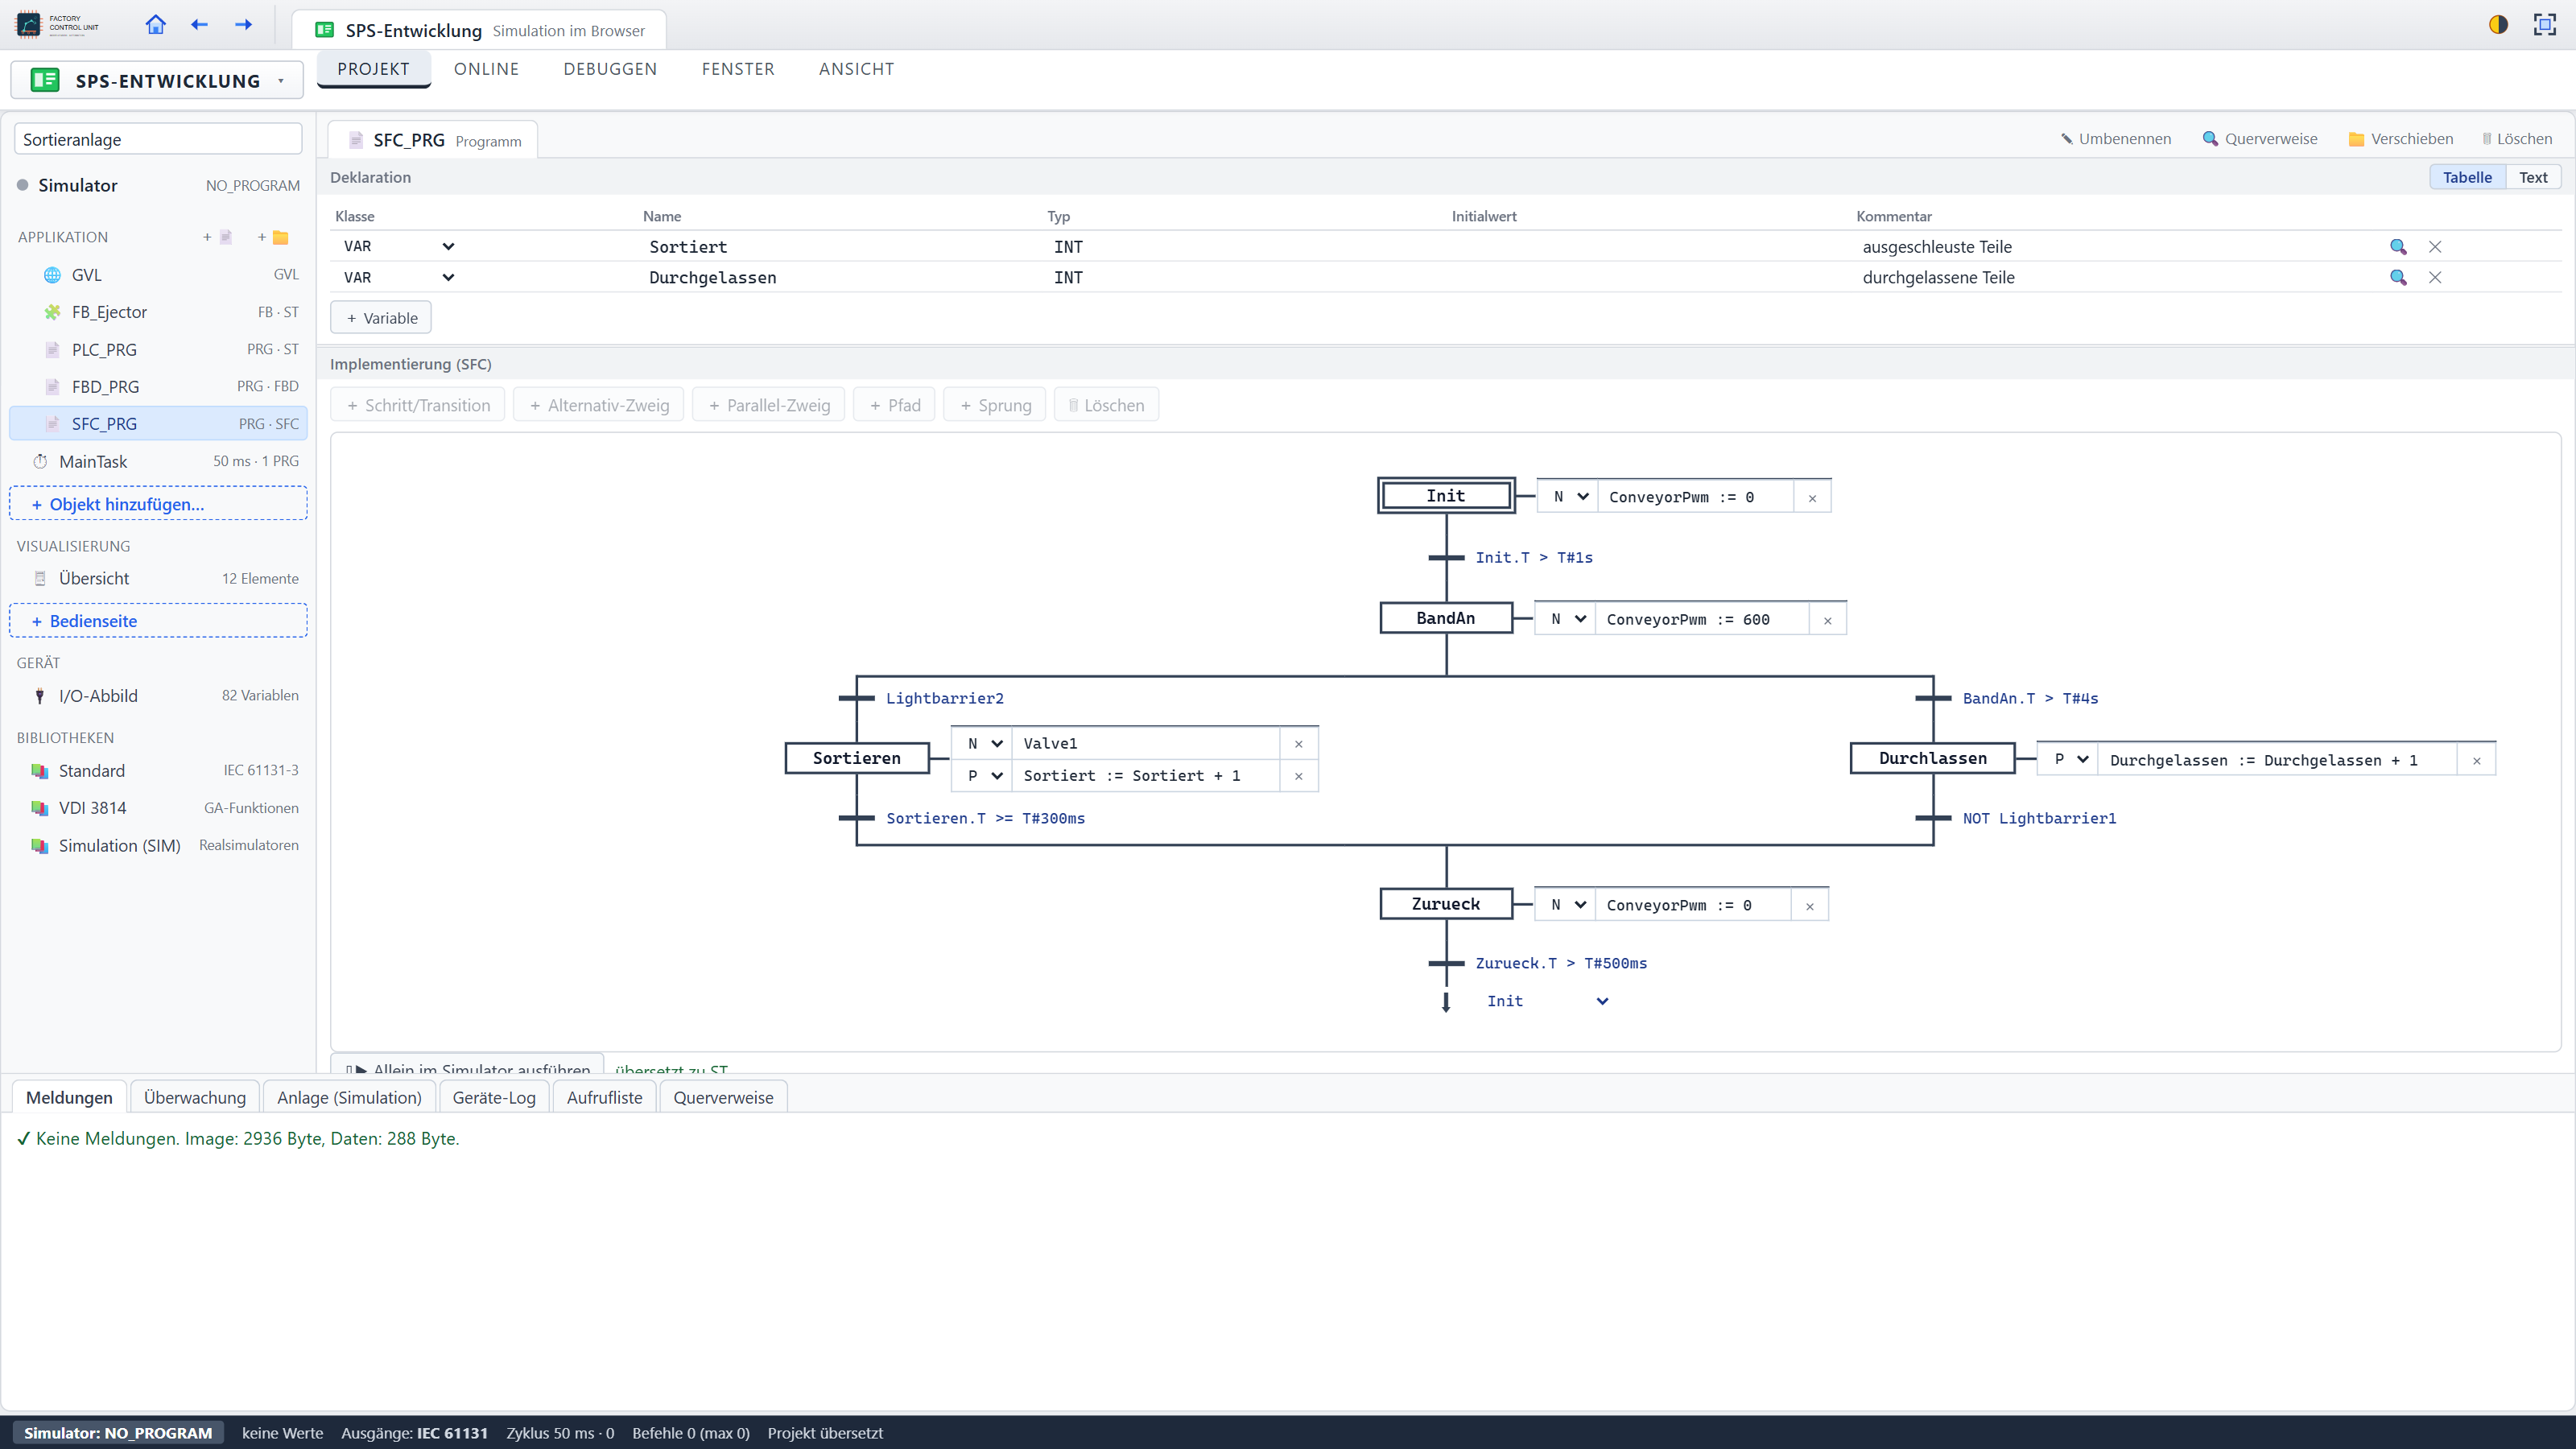
\includegraphics[width=\linewidth]{fig_sfc_editor.png}
\caption{Programmierumgebung im Browser: Ablaufsprache (AS) mit Projektbaum, Deklarationen und Werkzeugleiste; Sortierablauf mit Alternativverzweigung.}
\label{fig:sfc}
\end{figure}

\section{Einordnung: Softwareentwicklung mit KI}\label{sec:ki}

Noch vor wenigen Jahren wäre jeder einzelne der beschriebenen Bausteine eine eigene Veröffentlichung oder Abschlussarbeit wert gewesen: ein Echtzeitkernel mit vier CPU-Ports, ein IP-Stack, ein OPC-UA-Server mit Sicherheitsprofil, ein EtherCAT-Slave-Stack, ein USB-Stack, ein IEC-61131-3-Compiler mit zwei virtuellen Maschinen, ein Visualisierungssystem und präzise Peripheriemodelle für einen Emulator. Heute kann ein einzelner erfahrener Entwickler mit dem richtigen Prompting in wenigen Wochen eine solche Menge hochwertiger Software erstellen. Aus den Erfahrungen mit der FCU lassen sich vier Bedingungen ableiten, unter denen das gelingt.
\begin{itemize}
\item Anforderungen und Architektur bleiben Aufgabe des Menschen. Am Anfang stand eine präzise Systemvorgabe mit Designphilosophie, Zielplattform und Teststrategie. Eine projektweite Regeldatei hält verbindliche Konventionen fest und wächst mit dem Projekt.
\item Qualität entsteht durch ausführbare Nachweise, nicht durch das Lesen jeder Zeile. Testkette, Fuzzing und Penetrationstest sind die eigentliche Qualitätssicherung; die KI schreibt Code und Tests, abgenommen wird nur, was auf allen Stufen besteht.
\item Entscheidungen werden gemessen, nicht vermutet, wie bei der verworfenen TLS-Optimierung oder der Größe der Speicherpools.
\item Fachwissen bleibt nötig, um Irrwege zu erkennen: Zykluszahlen aus Emulatoren dürfen nicht als Hardwareleistung gelten; Stackgrößen müssen aus der Rahmenanalyse statt aus dem Emulator bestimmt werden, weil Renode die Stackgrenze nicht überwacht. Die Nutzung von C++26 deckte zudem einen Fehler in GCC 16 auf, der Contracts in bestimmten Fällen stillschweigend falsch übersetzt; er ist mit einem minimalen Beispiel dokumentiert und wird umgangen.
\end{itemize}

Grenzen bleiben: Es gibt keine formale Verifikation und keinen Sicherheitsanspruch im Sinne der funktionalen Sicherheit, und die Abhängigkeit von einem KI-Werkzeug ist ein eigenes Risiko. Für den Transfer ist zu beachten, dass rtoos unter der MIT-Lizenz steht, wolfSSL aber unter GPLv3 oder einer kommerziellen Lizenz.

\section{Einsatz in der Lehre und Ausblick}\label{sec:lehre}

Die FCU soll in vier Lehrveranstaltungen eingesetzt werden (Tabelle~\ref{tab:lehre}), die alle an derselben greifbaren Anlage, aber an unterschiedlichen Schnittstellen ansetzen.

\begin{table}[htbp]
\centering
\small
\caption{Geplanter Einsatz der FCU in vier Lehrveranstaltungen.}
\label{tab:lehre}
\begin{tabular}{p{0.20\linewidth}p{0.33\linewidth}p{0.41\linewidth}}
\toprule
\textbf{Veranstaltung} & \textbf{Lerninhalte} & \textbf{Nutzung der FCU} \\
\midrule
Connected Systems (Master) & Kommunikationsgrundlagen, Signierung und Verschlüsselung, Echtzeitprotokolle, IT-Sicherheit & Modbus, OPC UA (Sign, SignAndEncrypt) und EtherCAT auf einem Prozessmodell; Mitschnitte, Zertifikate, Fuzzing- und Pentest-Befunde \\[2pt]
Regelungstechnik & Streckenidentifikation, Reglerentwurf, Anti-Windup & Druckregelstrecke: Kennlinie, Sprungantwort, P/PI/PID-Regler einstellen und vergleichen \\[2pt]
Automatisierungs\-technik & IEC 61131-3, AS, FBS, ST, Bedienen und Beobachten & Integrierte Programmierumgebung im Browser oder Soft-SPS (z.\,B. CODESYS) über OPC UA, Modbus oder EtherCAT \\[2pt]
Embedded Systems & Hardwarenaher Entwurf, Echtzeitbetriebssystem, Treiber, Test & rtoos, Testkette mit Host, QEMU und Renode auch ohne Hardware; Baugruppe oder Treiber weiterentwickeln \\[2pt]
\bottomrule
\end{tabular}
\end{table}

Die Leistungsmessung mit dem INA226 erlaubt es, Ablaufvarianten energetisch zu vergleichen, und die Schrittmotortreiber senken den Spulenstrom lastabhängig. Ein verursachergerechtes Energiemonitoring ist jedoch nicht Gegenstand dieses Beitrags. Platinen der Revisionen 1 bis 3 sind aufgebaut, die Firmware läuft auf der Hardware. Als Nächstes folgen Aufgabenstellungen für alle vier Module und deren Erprobung mit Studierenden einschließlich einer Befragung. Hardware, Firmware und Weboberfläche werden unter offenen Lizenzen veröffentlicht.

\section{Literatur}

\bibliographystyle{unsrt}
\bibliography{references}

\end{document}
